\appendix
\section{Synthetic Datasets}\label{app:data}
\begin{figure}[ht]
    \centering
    \begin{subfigure}{0.45\textwidth}
        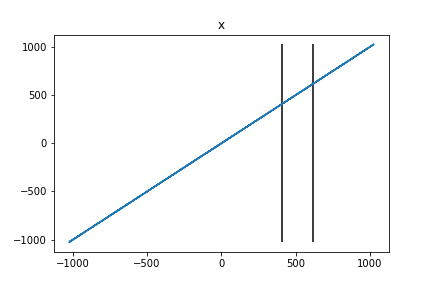
\includegraphics[width=\textwidth]{img/data_x.png}
    \end{subfigure}
    \begin{subfigure}{0.45\textwidth}
        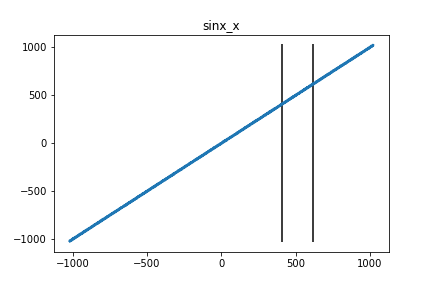
\includegraphics[width=\textwidth]{img/data_sinx_x.png}
    \end{subfigure}
    \begin{subfigure}{0.45\textwidth}
        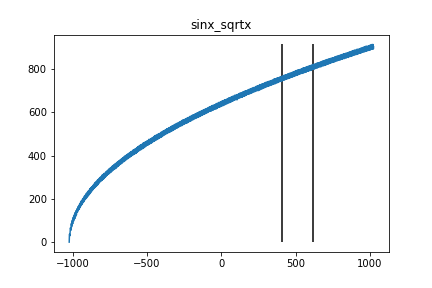
\includegraphics[width=\textwidth]{img/data_sinx_sqrtx.png}
    \end{subfigure}
    \begin{subfigure}{0.45\textwidth}
        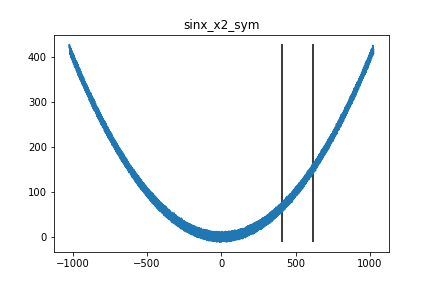
\includegraphics[width=\textwidth]{img/data_sinx_x2_sym.png}
    \end{subfigure}
    \begin{subfigure}{0.45\textwidth}
        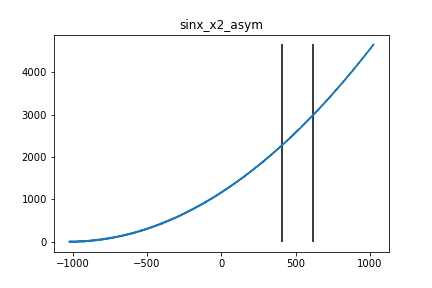
\includegraphics[width=\textwidth]{img/data_sinx_x2_asym.png}
    \end{subfigure}
    \caption{Synthetic datasets with underlying trend. 
    The entire datasets are plotted, so the cyclical patterns by \texttt{sin} function is not visually identifiable. 
    The black vertical lines split the the training, development and test datasets, from left to right.}
\end{figure}

\begin{figure}[ht]
    \centering
    \begin{subfigure}{0.45\textwidth}
        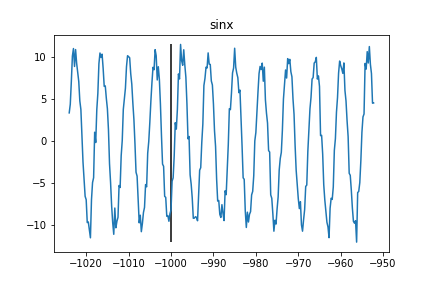
\includegraphics[width=\textwidth]{img/data_sinx.png}
    \end{subfigure}
    \begin{subfigure}{0.45\textwidth}
        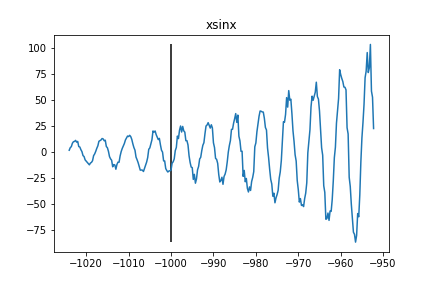
\includegraphics[width=\textwidth]{img/data_xsinx.png}
    \end{subfigure}
    \begin{subfigure}{0.45\textwidth}
        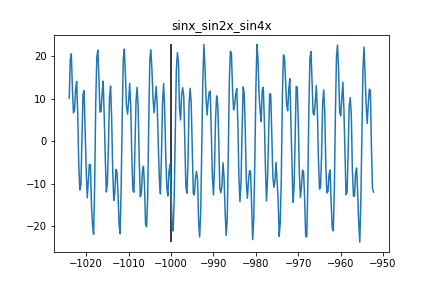
\includegraphics[width=\textwidth]{img/data_sinx_sin2x_sin4x.png}
    \end{subfigure}
    \begin{subfigure}{0.45\textwidth}
        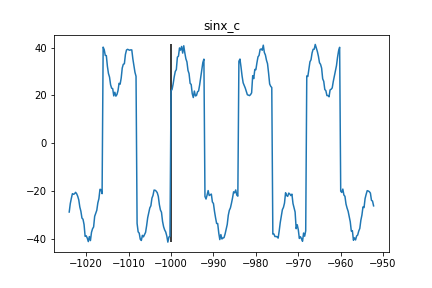
\includegraphics[width=\textwidth]{img/data_sinx_c.png}
    \end{subfigure}
    \caption{Synthetic datasets without underlying trend. 
    Only one subsequence is plotted, where the black vertical line splits the encoder input and forecasting target.}
\end{figure}
\clearpage


\section{Prediction Plots}\label{app:pred}
\begin{figure}[ht]
    \centering
    \begin{subfigure}{0.75\textwidth}
        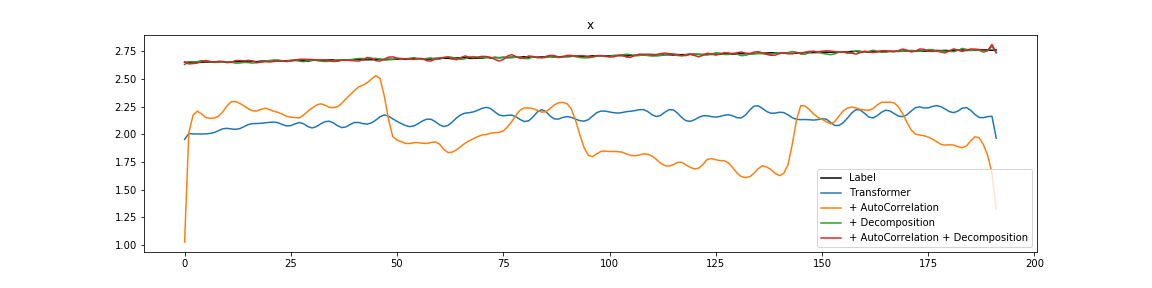
\includegraphics[width=\textwidth]{img/pred_x.png}
    \end{subfigure}
    \begin{subfigure}{0.75\textwidth}
        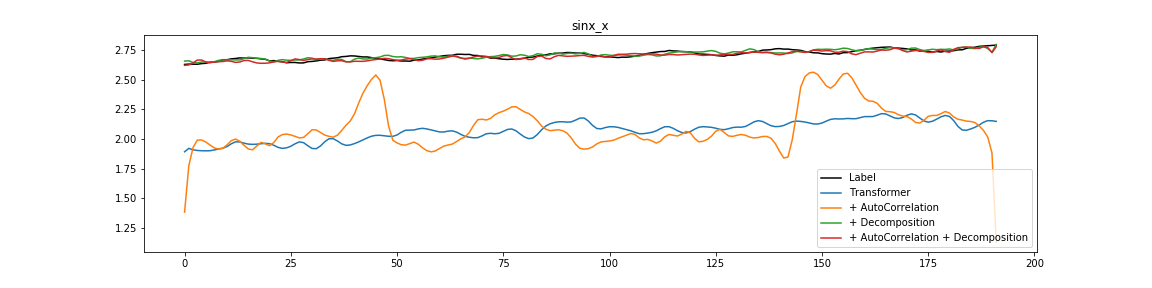
\includegraphics[width=\textwidth]{img/pred_sinx_x.png}
    \end{subfigure}
    \begin{subfigure}{0.75\textwidth}
        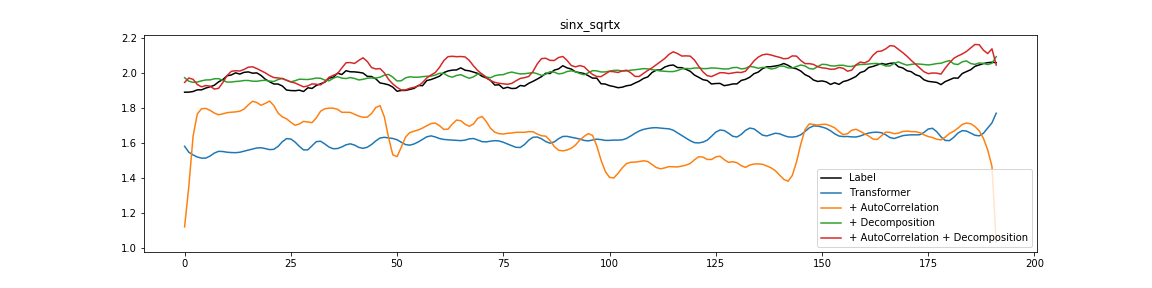
\includegraphics[width=\textwidth]{img/pred_sinx_sqrtx.png}
    \end{subfigure}
    \begin{subfigure}{0.75\textwidth}
        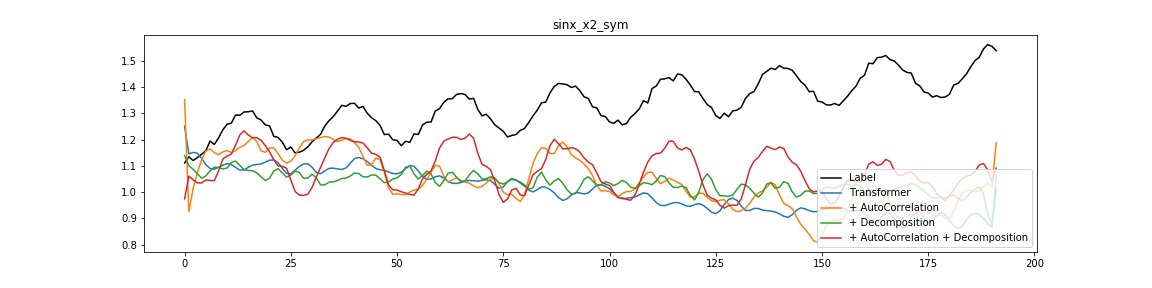
\includegraphics[width=\textwidth]{img/pred_sinx_x2_sym.png}
    \end{subfigure}
    \begin{subfigure}{0.75\textwidth}
        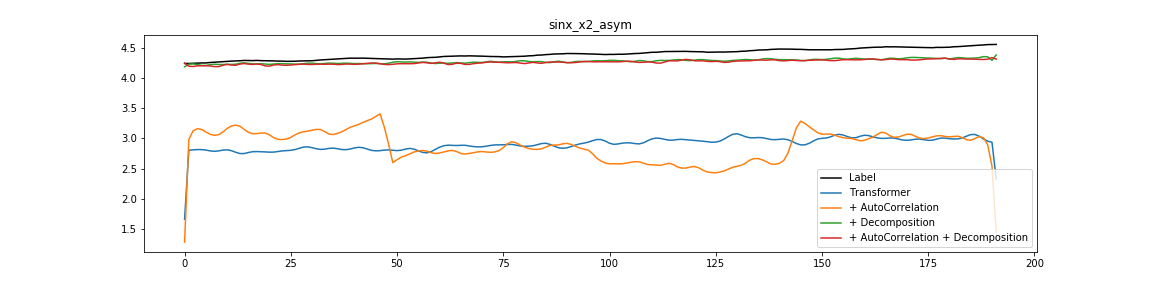
\includegraphics[width=\textwidth]{img/pred_sinx_x2_asym.png}
    \end{subfigure}
    \caption{Forecasting one subsequence in synthetic datasets with underlying trend.}
\end{figure}

\begin{figure}[ht]
    \centering
    \begin{subfigure}{0.75\textwidth}
        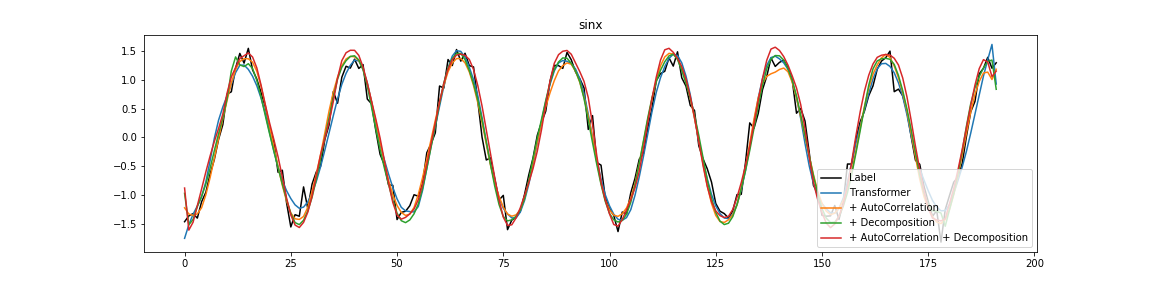
\includegraphics[width=\textwidth]{img/pred_sinx.png}
    \end{subfigure}
    \begin{subfigure}{0.75\textwidth}
        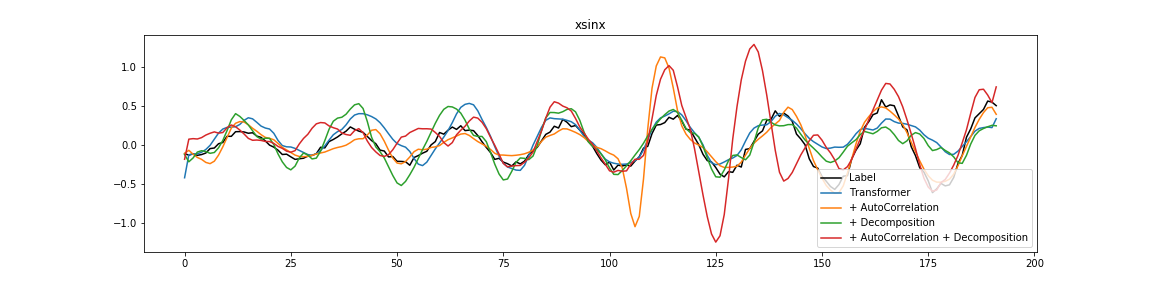
\includegraphics[width=\textwidth]{img/pred_xsinx.png}
    \end{subfigure}
    \begin{subfigure}{0.75\textwidth}
        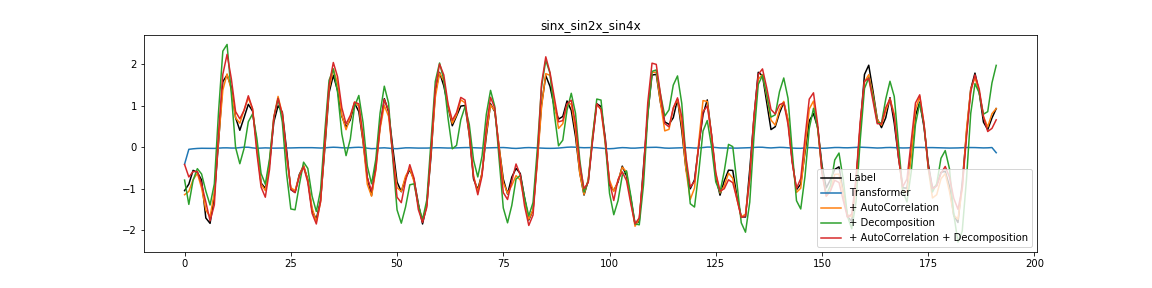
\includegraphics[width=\textwidth]{img/pred_sinx_sin2x_sin4x.png}
    \end{subfigure}
    \begin{subfigure}{0.75\textwidth}
        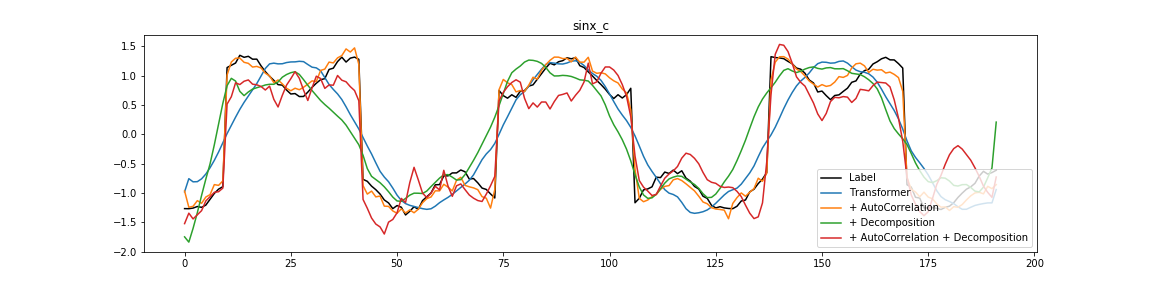
\includegraphics[width=\textwidth]{img/pred_sinx_c.png}
    \end{subfigure}
    \caption{Forecasting one subsequence in synthetic datasets without underlying trend.}
\end{figure}

\begin{figure}[ht]
    \centering
    \begin{subfigure}{0.6\textwidth}
        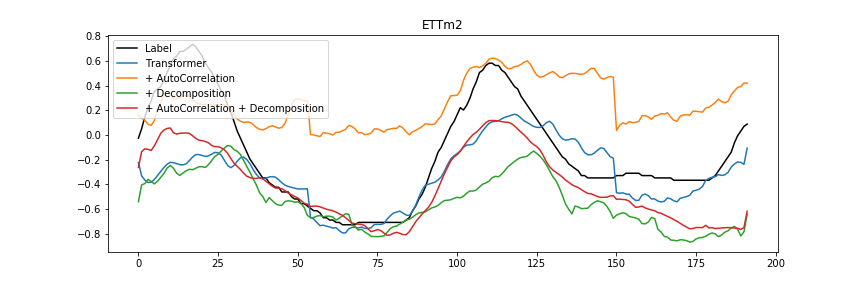
\includegraphics[width=\textwidth]{img/pred_ETTm2.png}
    \end{subfigure}
    \begin{subfigure}{0.6\textwidth}
        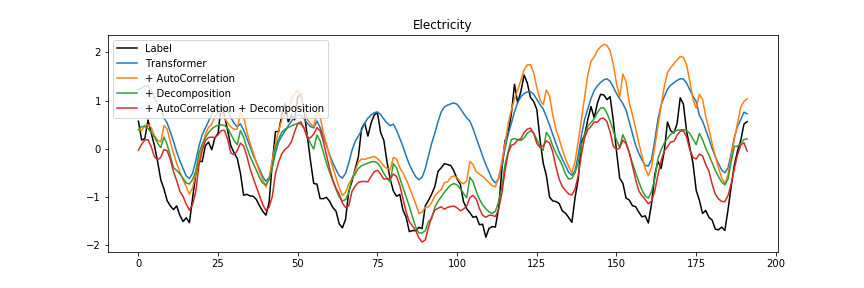
\includegraphics[width=\textwidth]{img/pred_Electricity.png}
    \end{subfigure}
    \begin{subfigure}{0.6\textwidth}
        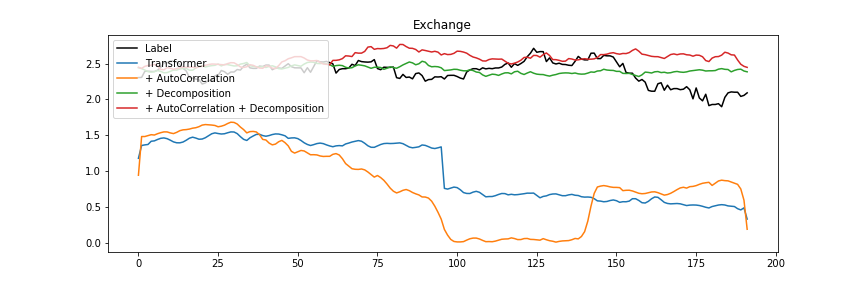
\includegraphics[width=\textwidth]{img/pred_Exchange.png}
    \end{subfigure}
    \begin{subfigure}{0.6\textwidth}
        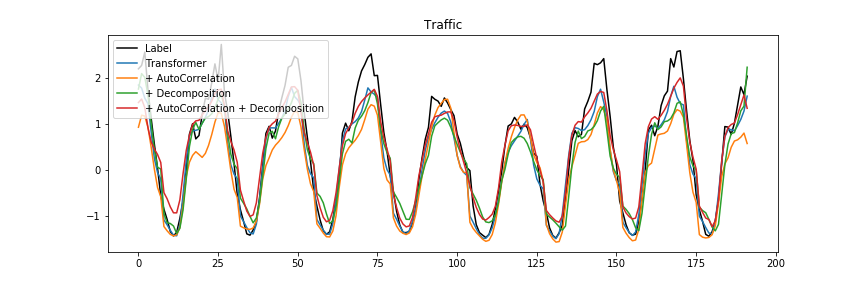
\includegraphics[width=\textwidth]{img/pred_Traffic.png}
    \end{subfigure}
    \begin{subfigure}{0.6\textwidth}
        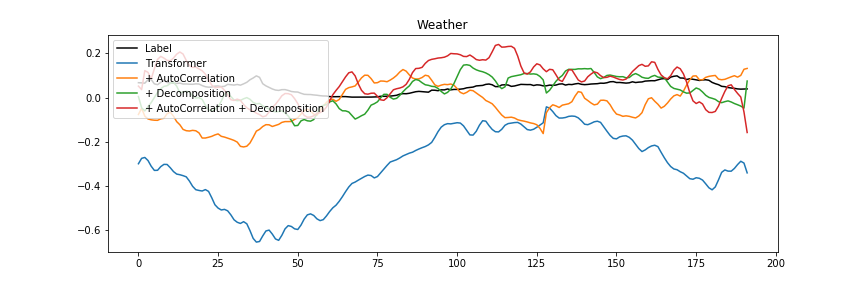
\includegraphics[width=\textwidth]{img/pred_Weather.png}
    \end{subfigure}
    \begin{subfigure}{0.6\textwidth}
        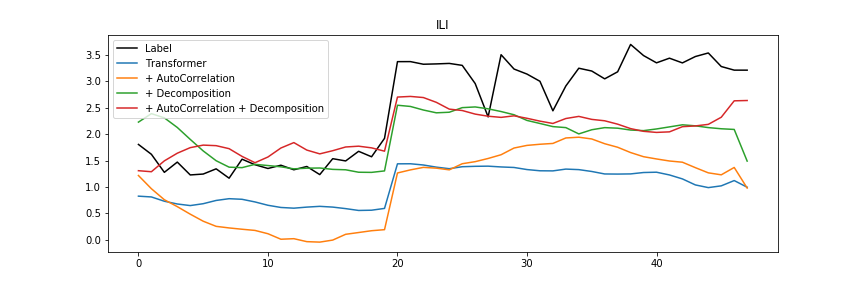
\includegraphics[width=\textwidth]{img/pred_ILI.png}
    \end{subfigure}
    \caption{Forecasting one subsequence in synthetic datasets without underlying trend.}
\end{figure}
\clearpage


\section{AutoCorrelation Weights}\label{app:tau}
\begin{figure}[ht]
    \centering
    \begin{subfigure}{\textwidth}
        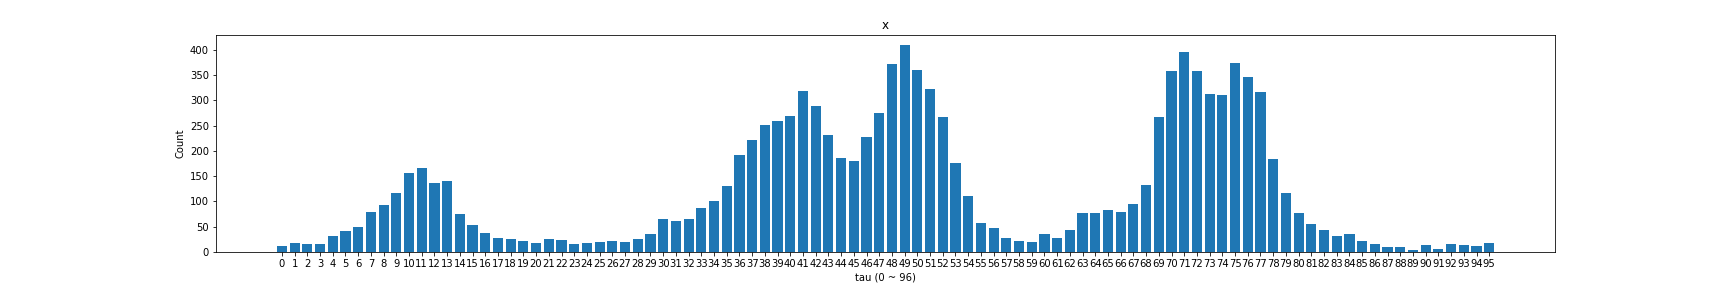
\includegraphics[width=\textwidth]{img/tau_x.png}
    \end{subfigure}
    \begin{subfigure}{\textwidth}
        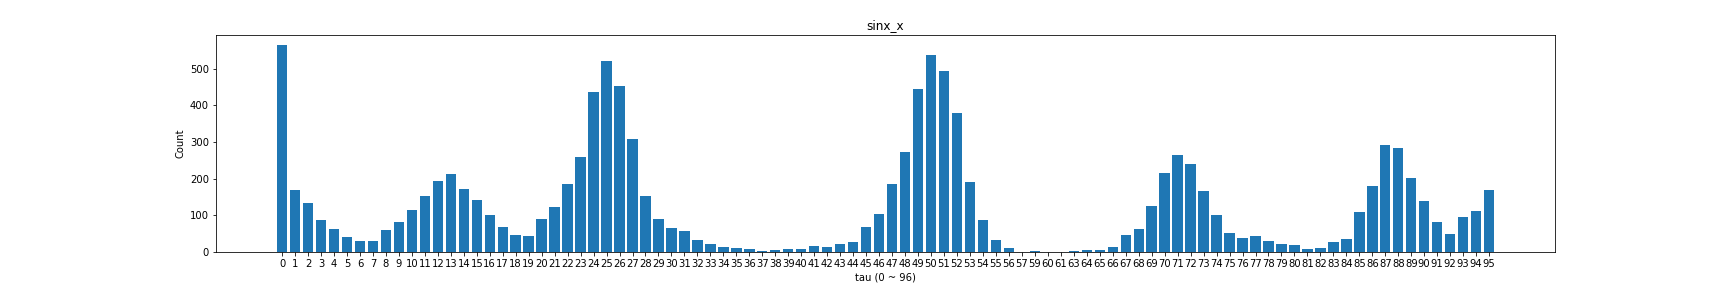
\includegraphics[width=\textwidth]{img/tau_sinx_x.png}
    \end{subfigure}
    \begin{subfigure}{\textwidth}
        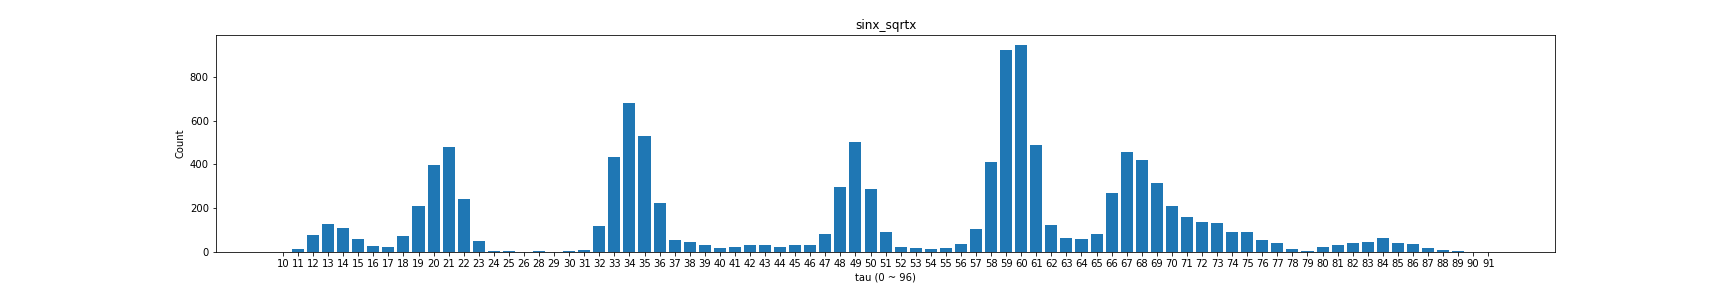
\includegraphics[width=\textwidth]{img/tau_sinx_sqrtx.png}
    \end{subfigure}
    \begin{subfigure}{\textwidth}
        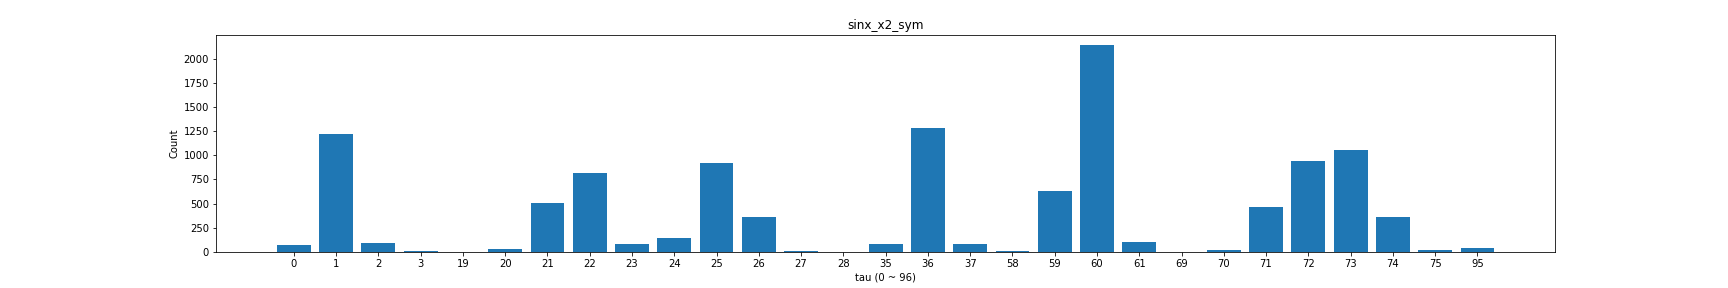
\includegraphics[width=\textwidth]{img/tau_sinx_x2_sym.png}
    \end{subfigure}
    \begin{subfigure}{\textwidth}
        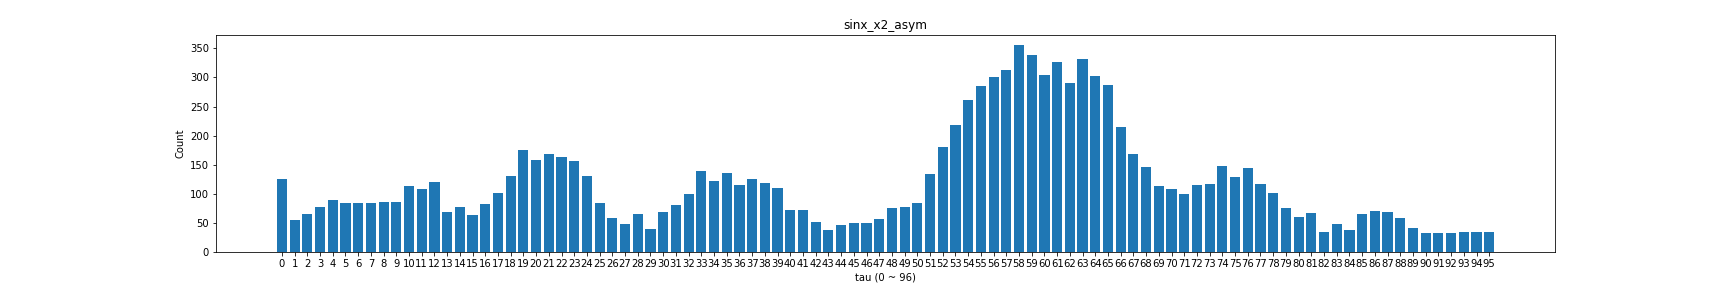
\includegraphics[width=\textwidth]{img/tau_sinx_x2_asym.png}
    \end{subfigure}
    \caption{Distributions of $\tau$ on synthetic datasets with trend.}
\end{figure}

\begin{figure}[ht]
    \centering
    \begin{subfigure}{\textwidth}
        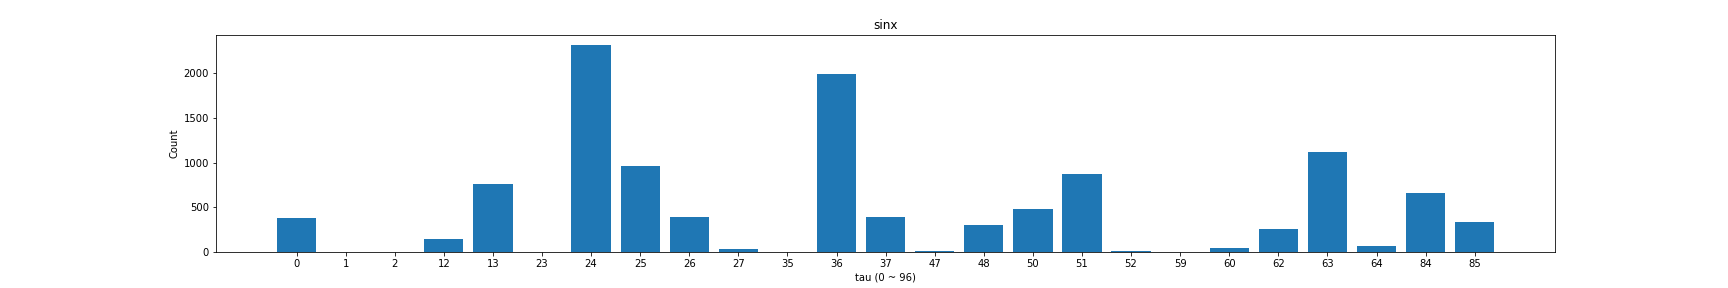
\includegraphics[width=\textwidth]{img/tau_sinx.png}
    \end{subfigure}
    \begin{subfigure}{\textwidth}
        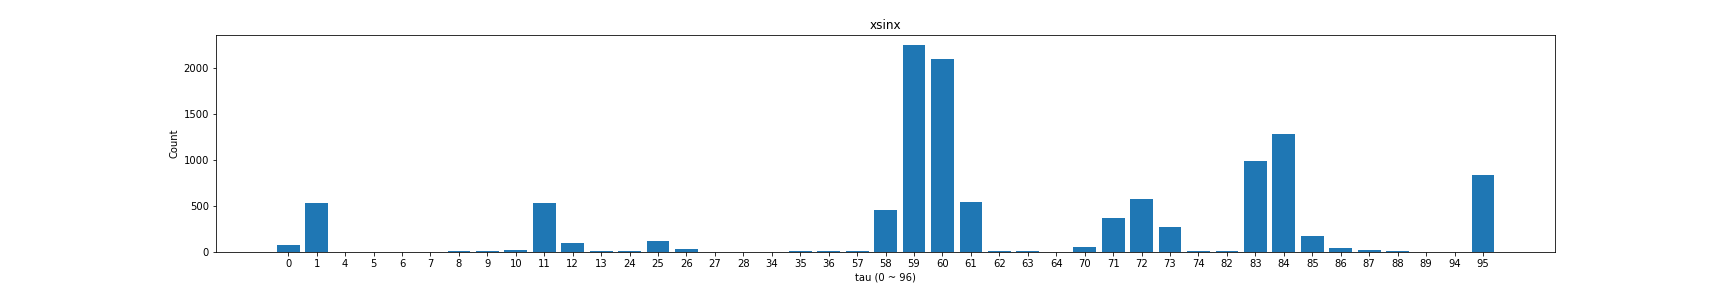
\includegraphics[width=\textwidth]{img/tau_xsinx.png}
    \end{subfigure}
    \begin{subfigure}{\textwidth}
        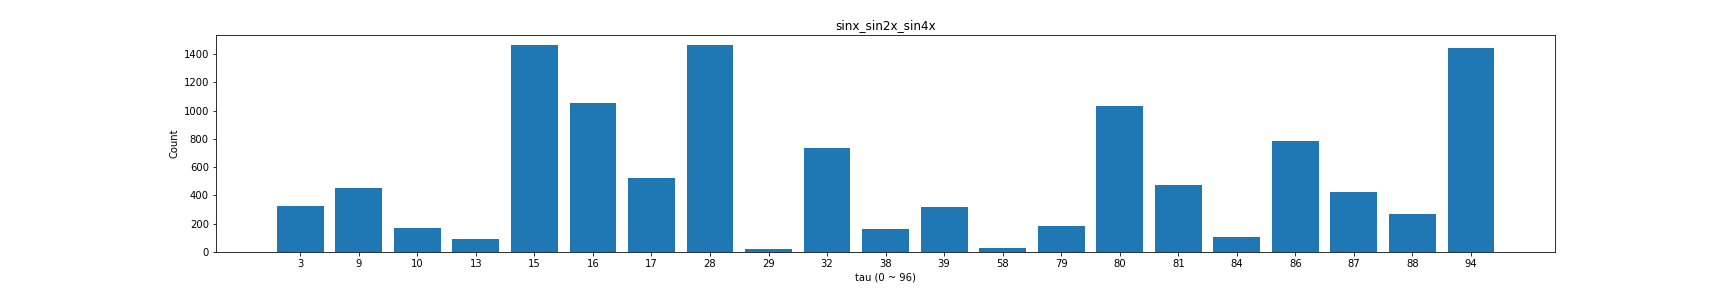
\includegraphics[width=\textwidth]{img/tau_sinx_sin2x_sin4x.png}
    \end{subfigure}
    \begin{subfigure}{\textwidth}
        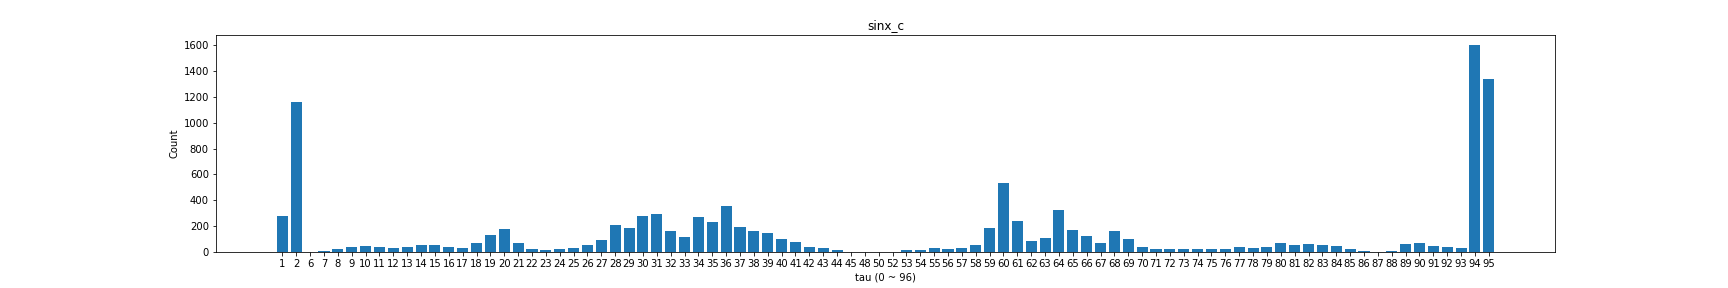
\includegraphics[width=\textwidth]{img/tau_sinx_c.png}
    \end{subfigure}
    \caption{Distributions of $\tau$ on synthetic datasets without trend.}
\end{figure}
